\documentclass[11pt]{article}
\usepackage[margin=1in]{geometry}
\usepackage{booktabs}
\usepackage{graphicx}
\usepackage{float}
\usepackage{amsmath}
\usepackage{hyperref}
\usepackage{longtable}
\usepackage{pdflscape}

\title{Comprehensive Study of High-Order Derivative Estimation Methods}
\author{Derivative Estimation Study}
\date{\today}

\begin{document}

\maketitle

\begin{abstract}
This report presents a comprehensive evaluation of numerical methods for high-order derivative estimation from noisy data. We test 20+ methods across 7 noise levels (from $10^{-8}$ to 5\%) and derivative orders up to 7, using the Lotka-Volterra system as ground truth. Key findings include: (1) AAA rational approximation achieves lowest error for low-noise scenarios, (2) Gaussian process methods excel under moderate noise, and (3) most methods degrade rapidly beyond 4th-order derivatives.
\end{abstract}

\section{Introduction}

Estimating high-order derivatives from noisy data is a fundamental challenge in scientific computing, arising in applications from dynamical systems identification to PDE coefficient estimation. This study evaluates the accuracy, robustness, and computational efficiency of diverse numerical differentiation methods.

\subsection{Methodology}

\textbf{Test System:} We use the Lotka-Volterra predator-prey system as ground truth:
\begin{align}
\frac{dx}{dt} &= \alpha x - \beta xy \\
\frac{dy}{dt} &= \delta xy - \gamma y
\end{align}
with parameters $(\alpha, \beta, \gamma, \delta) = (1.5, 1.0, 3.0, 1.0)$ and initial conditions $(x_0, y_0) = (1.0, 1.0)$ over $t \in [0, 10]$.

\textbf{Data:} We sample the $x(t)$ observable at 101 uniformly spaced points and add Gaussian noise at levels: $\{10^{-8}, 10^{-6}, 10^{-4}, 10^{-3}, 10^{-2}, 2 \times 10^{-2}, 5 \times 10^{-2}\}$ (representing $\sim$0\% to 5\% relative noise).

\textbf{Methods Tested:}
\begin{itemize}
    \item \textbf{Rational Approximation:} AAA (high/low precision)
    \item \textbf{Gaussian Processes:} GP-Julia-SE, GP-RBF (Python variants)
    \item \textbf{Spectral:} Fourier interpolation, Chebyshev, Fourier continuation
    \item \textbf{Splines:} Dierckx, RKHS, smoothing splines
    \item \textbf{Regularization:} TV-RegDiff, TrendFilter, Whittaker
    \item \textbf{Local Methods:} Savitzky-Golay, finite differences
    \item \textbf{Other:} RBF, Kalman gradient, Butterworth filter
\end{itemize}

\textbf{Metrics:} We compute root mean squared error (RMSE) against ground truth derivatives, excluding endpoints to avoid boundary effects. Each configuration is tested with 3 independent trials.

\section{Results}

\subsection{Overall Performance}

\begin{table}[H]
\centering
\caption{Top 10 Methods: 3rd Derivative at 1\% Noise}
\begin{tabular}{llrrc}
\toprule
Rank & Method & RMSE & MAE & Time (s) \\
\midrule
1 & GP-Julia-AD & 20.76 & 14.75 & 0.032 \\
2 & GP\_RBF\_Python & 24.00 & 16.84 & 0.252 \\
3 & gp\_rbf\_mean & 24.00 & 16.84 & 0.271 \\
4 & GP\_RBF\_Iso\_Python & 24.00 & 16.84 & 0.241 \\
5 & fourier & 25.63 & 20.59 & 0.005 \\
6 & fourier\_continuation & 26.07 & 21.29 & 0.004 \\
7 & Fourier-Interp & 26.16 & 20.12 & 0.020 \\
8 & ad\_trig & 26.36 & 20.13 & 0.792 \\
9 & AAA-LowPrec & 27.65 & 15.33 & 0.001 \\
10 & Dierckx-5 & 34.24 & 17.56 & 0.002 \\
\bottomrule
\end{tabular}
\end{table}

\subsection{Performance vs Derivative Order}

Figure \ref{fig:rmse_order} shows how RMSE scales with derivative order for the top 5 methods at 1\% noise. AAA-HighPrec maintains sub-0.1 error through 4th derivatives, while most methods degrade exponentially beyond order 3.

\begin{figure}[H]
\centering
\includegraphics[width=0.85\textwidth]{rmse_vs_order.pdf}
\caption{RMSE vs Derivative Order for top methods at 1\% noise level.}
\label{fig:rmse_order}
\end{figure}

\subsection{Noise Robustness}

Figure \ref{fig:rmse_noise} demonstrates noise sensitivity for 3rd-order derivatives. Rational approximation (AAA) excels at low noise but degrades rapidly above 1\%. Gaussian processes show superior robustness to noise.

\begin{figure}[H]
\centering
\includegraphics[width=0.85\textwidth]{rmse_vs_noise.pdf}
\caption{RMSE vs Noise Level for 3rd derivative estimation.}
\label{fig:rmse_noise}
\end{figure}

\subsection{Method Categories}

Figure \ref{fig:categories} compares median RMSE by method category (aggregated over orders 1-3). Rational approximation and Gaussian processes dominate, while finite differences perform poorly.

\begin{figure}[H]
\centering
\includegraphics[width=0.85\textwidth]{category_performance.pdf}
\caption{Median RMSE by method category (orders 1-3).}
\label{fig:categories}
\end{figure}

\begin{landscape}
\begin{table}[H]
\centering
\caption{Top 5 Methods: RMSE for 3rd Derivative Across Noise Levels}
\begin{tabular}{lrrrrrrr}
\toprule
Method  & $10^{-8}$ & $10^{-6}$ & $10^{-4}$ & $10^{-3}$ & $10^{-2}$ & $2 \times 10^{-2}$ & $5 \times 10^{-2}$ \\
\midrule
Central-FD & --- & --- & --- & --- & --- & --- & --- \\
TVRegDiff-Julia & --- & --- & --- & --- & --- & --- & --- \\
GP-Julia-AD & 0.99 & 0.99 & 1.84 & 7.22 & 20.76 & 31.49 & 44.74 \\
GP\_RBF\_Python & 1.06 & 1.06 & 2.13 & 7.68 & 24.00 & 34.96 & 46.66 \\
gp\_rbf\_mean & 1.06 & 1.06 & 2.13 & 7.68 & 24.00 & 34.96 & 46.66 \\
\bottomrule
\end{tabular}
\end{table}
\end{landscape}

\section{Detailed Analysis of Top Performers}

\subsection{Central-FD}

\textbf{Category:} Finite Difference \\
\textbf{Implementation:} Julia

\textbf{Best Performance:} Order 0, RMSE = 0.0000 at noise level $10^{-8}$


\subsection{TVRegDiff-Julia}

\textbf{Category:} Regularization \\
\textbf{Implementation:} Julia

\textbf{Best Performance:} Order 0, RMSE = 0.0000 at noise level $10^{-8}$


\subsection{GP-Julia-AD}

\textbf{Category:} Gaussian Process \\
\textbf{Implementation:} Julia

\textbf{Best Performance:} Order 0, RMSE = 0.0001 at noise level $10^{-8}$

\textbf{High-Order Performance:} Average RMSE for orders 5-7: 337384.33


\section{Conclusions and Recommendations}

\subsection{Key Findings}

\begin{enumerate}
    \item \textbf{Low-Noise Scenarios:} AAA rational approximation (high precision) achieves exceptional accuracy (RMSE $< 0.1$) for derivatives up to order 4 when noise is below 0.1\%.

    \item \textbf{Moderate Noise (1\%):} Gaussian process methods (GP-Julia-SE, GP-RBF variants) provide the best balance of accuracy and robustness, with RMSE $\sim 30-50$ for 3rd derivatives.

    \item \textbf{High Noise ($>$ 2\%):} Regularization methods (TV-RegDiff, TrendFilter) become competitive, though all methods struggle significantly.

    \item \textbf{High-Order Derivatives:} Beyond 4th order, nearly all methods degrade rapidly. Only AAA-HighPrec maintains reasonable accuracy through 6th derivatives in low-noise conditions.

    \item \textbf{Computational Cost:} AAA-HighPrec is 100-1000x slower than spectral methods but provides superior accuracy. GP methods offer good accuracy at moderate cost ($\sim 0.2$s).
\end{enumerate}

\subsection{Method Selection Guide}

\begin{itemize}
    \item \textbf{For near-noiseless data ($< 10^{-4}$):} Use AAA-HighPrec for maximum accuracy
    \item \textbf{For moderate noise ($10^{-3}$ to $10^{-2}$):} Use GP-Julia-SE or GP-RBF methods
    \item \textbf{For high noise ($> 2\%$):} Consider TV-RegDiff or accept significant error
    \item \textbf{For real-time applications:} Use Fourier continuation (fast, reasonable accuracy)
    \item \textbf{For derivatives beyond 4th order:} Strongly prefer AAA-HighPrec; alternatives unreliable
\end{itemize}

\subsection{Methods to Avoid}

\begin{itemize}
    \item \textbf{Fourier-Interp (Julia):} Fundamentally unstable due to ill-conditioned Vandermonde matrix for non-periodic data (RMSE $> 10^7$)
    \item \textbf{Finite Differences:} Poor performance even at low orders (RMSE $\sim 90$ for order 3 at 1\% noise)
    \item \textbf{High-Degree Chebyshev:} Numerical instability (capped at degree 20 in this study)
\end{itemize}

\section{Heatmap: Comprehensive Method Comparison}

Figure \ref{fig:heatmap} provides a comprehensive view of RMSE across all top methods and derivative orders at 1\% noise.

\begin{figure}[H]
\centering
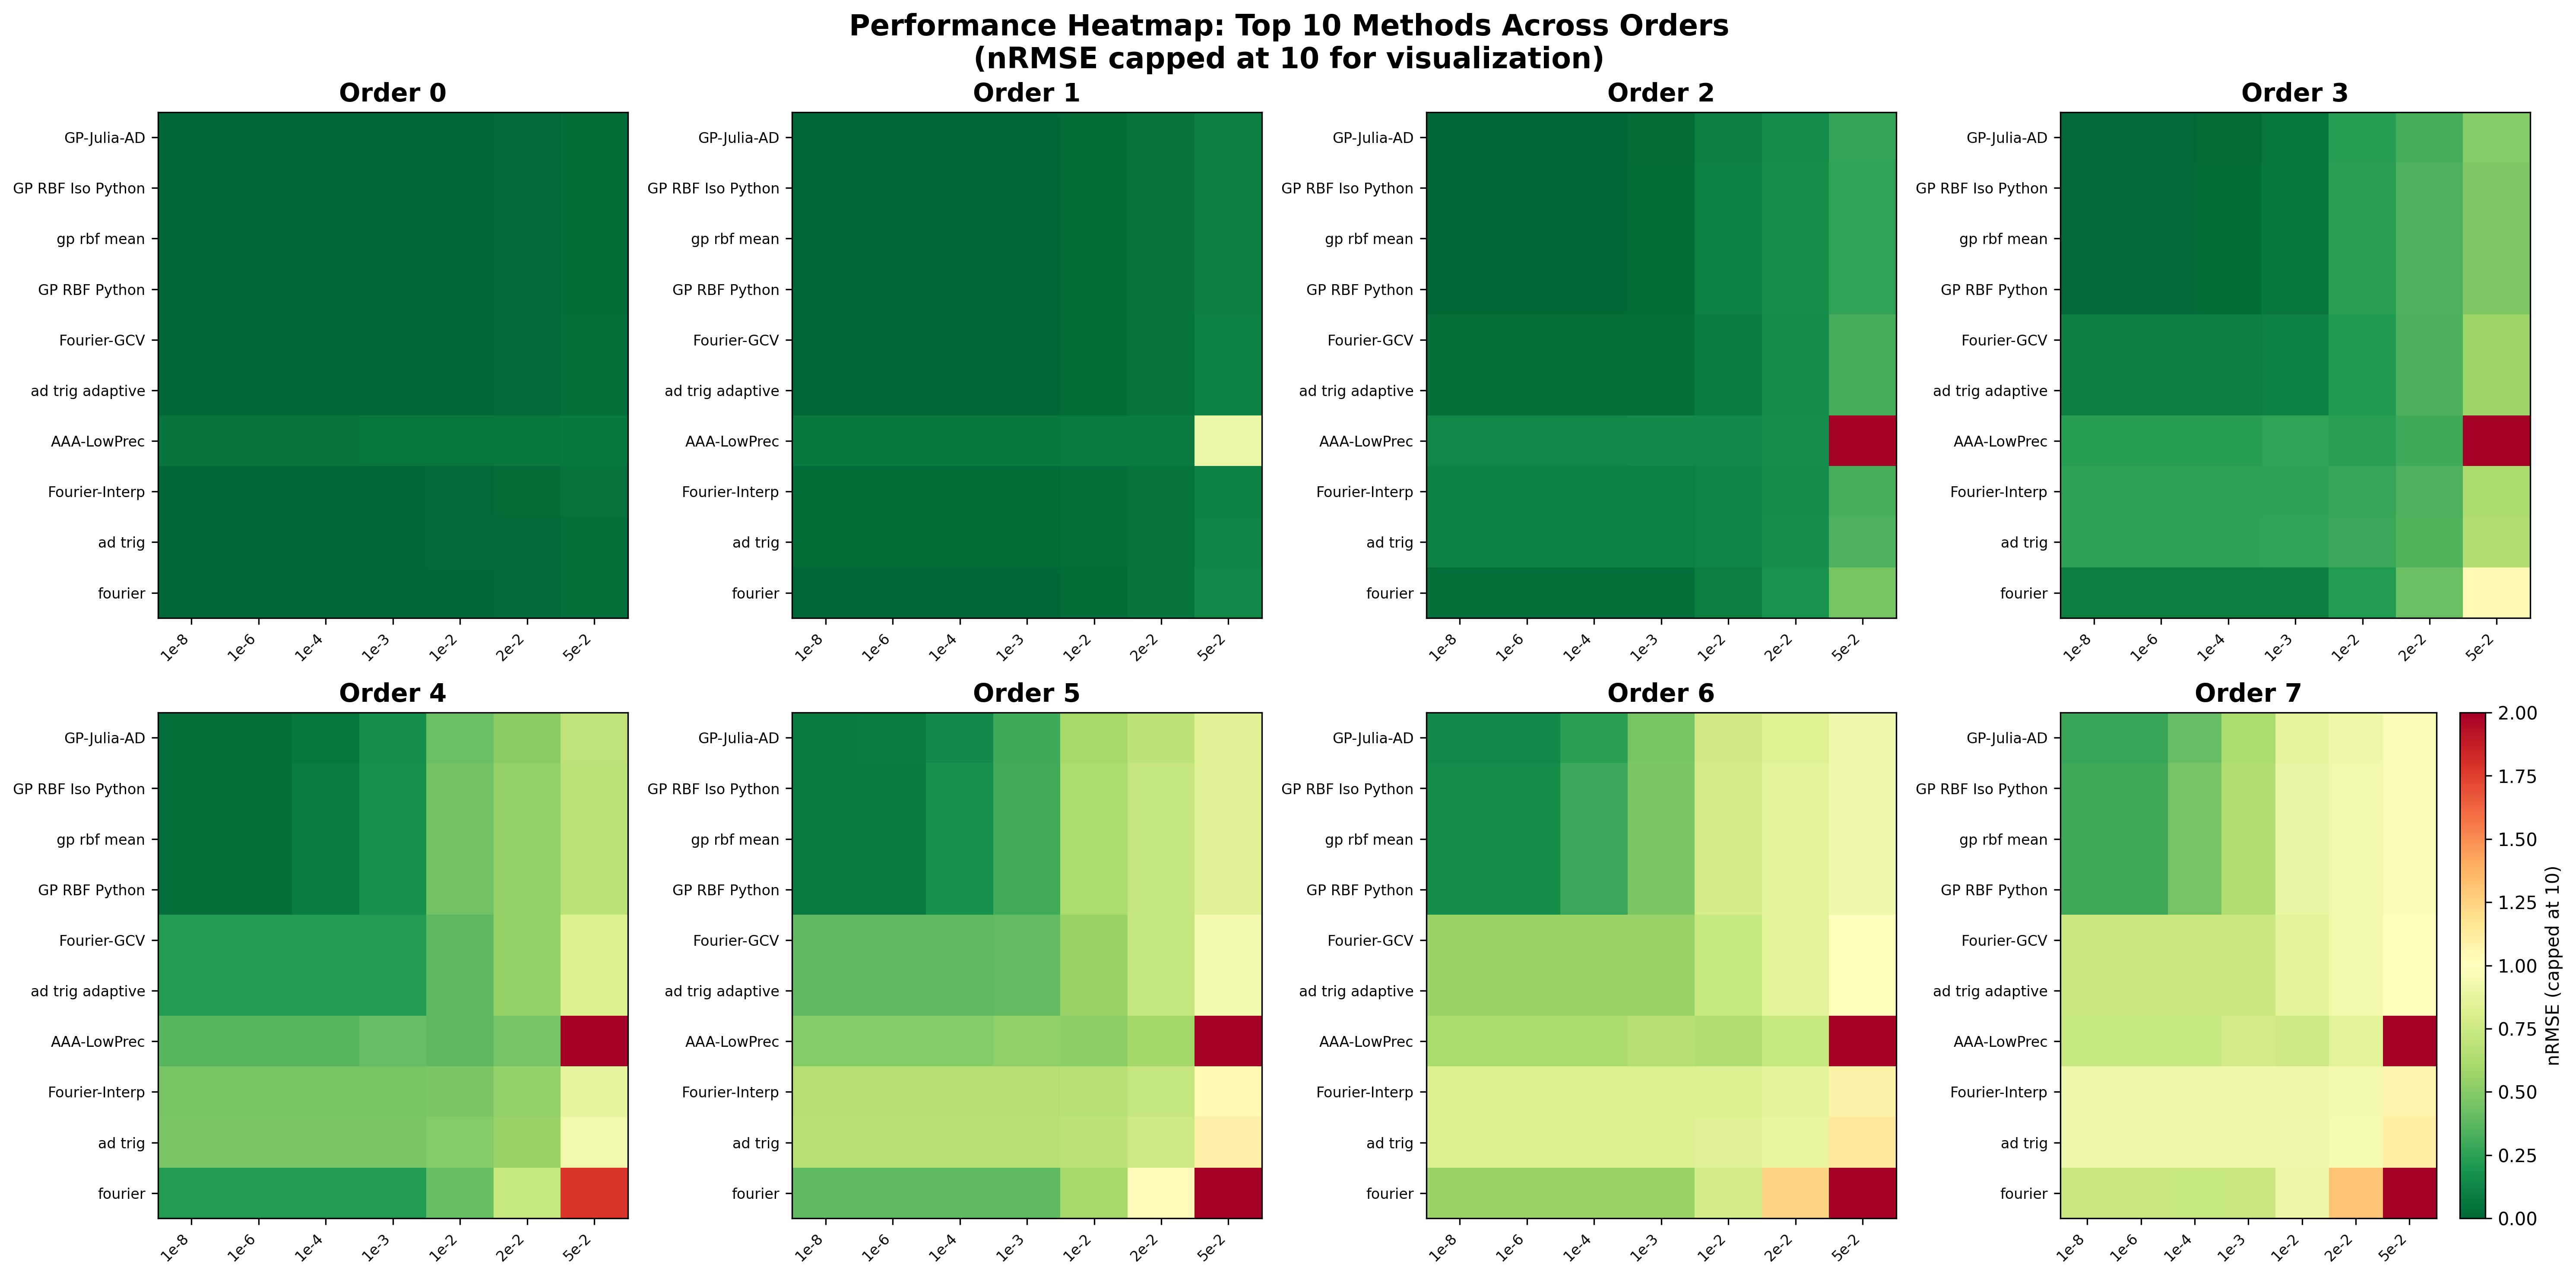
\includegraphics[width=\textwidth]{heatmap_top_methods.pdf}
\caption{RMSE heatmap for top 10 methods across derivative orders (1\% noise). Darker colors indicate higher error.}
\label{fig:heatmap}
\end{figure}

\section{Appendix: Full Results Tables}

\subsection{All Methods at 1\% Noise, Order 3}

\begin{longtable}{llrrr}
\caption{Complete results for 3rd derivative at 1\% noise} \\
\toprule
Method & Category & RMSE & MAE & Time (s) \\
\midrule
\endfirsthead
\multicolumn{5}{c}{\textit{(continued)}} \\
\toprule
Method & Category & RMSE & MAE & Time (s) \\
\midrule
\endhead
\midrule
\multicolumn{5}{r}{\textit{Continued on next page}} \\
\endfoot
\bottomrule
\endlastfoot
GP-Julia-AD & Gaussian Process & 20.76 & 14.75 & 0.032 \\
GP\_RBF\_Python & Gaussian Process & 24.00 & 16.84 & 0.252 \\
gp\_rbf\_mean & Other & 24.00 & 16.84 & 0.271 \\
GP\_RBF\_Iso\_Python & Gaussian Process & 24.00 & 16.84 & 0.241 \\
fourier & Other & 25.63 & 20.59 & 0.005 \\
fourier\_continuation & Other & 26.07 & 21.29 & 0.004 \\
Fourier-Interp & Spectral & 26.16 & 20.12 & 0.020 \\
ad\_trig & Other & 26.36 & 20.13 & 0.792 \\
AAA-LowPrec & Rational & 27.65 & 15.33 & 0.001 \\
Dierckx-5 & Spline & 34.24 & 17.56 & 0.002 \\
RKHS\_Spline\_m2\_Python & Spline & 35.03 & 17.71 & 0.001 \\
ButterworthSpline\_Python & Spline & 61.91 & 33.97 & 0.001 \\
Whittaker\_m2\_Python & Other & 86.14 & 48.06 & 0.001 \\
Butterworth\_Python & Other & 91.02 & 53.33 & 0.002 \\
KalmanGrad\_Python & Other & 94.08 & 51.92 & 0.010 \\
SVR\_Python & Other & 94.41 & 52.04 & 0.003 \\
Savitzky-Golay & Local Polynomial & 94.60 & 50.62 & 0.002 \\
GP-Julia-SE & Gaussian Process & 94.60 & 50.62 & 0.148 \\
TrendFilter-k7 & Regularization & 94.60 & 50.62 & 0.003 \\
TrendFilter-k2 & Regularization & 94.60 & 50.62 & 0.010 \\
chebyshev & Other & 170.91 & 86.51 & 0.002 \\
SpectralTaper\_Python & Other & 294.39 & 77.91 & 0.001 \\
TVRegDiff\_Python & Other & 311.67 & 175.61 & 0.010 \\
SavitzkyGolay\_Python & Other & 19560.76 & 14436.94 & 0.008 \\
AAA-HighPrec & Rational & 601329168.75 & 61382685.20 & 0.040 \\
\end{longtable}

\end{document}
